\documentclass[12pt]{article}
\usepackage{hyperref}
\usepackage{listings}
\usepackage{biblatex}
\usepackage{tikz}
\usepackage{refstyle}
\usepackage{mathabx}
%\usepackage{amssymb}
\usepackage{caption}
\usepackage{float}
\usepackage{graphicx}
\usepackage{graphics}
\usepackage{subfig}

\graphicspath{{/storage/self/primary/Download/latexnew/fig}}
\begin{document}
\title{\textbf{AVR-GCC}}
\date{}
\maketitle
\begin{enumerate}
    \item \textbf{Question(GATE-IN-2018-17):}For the 3-bit binary counter shown in the figure, the output increments at every positive 
transition in the clock (CLK). Assume ideal diodes and the starting state of the counter as 
000. If output high is 1 V and output low is 0 V, the current I (in mA) flowing through the 
50 Ω resistor during the 5th clock cycle is (up to one decimal place)

 \begin{figure}[H]
\centering
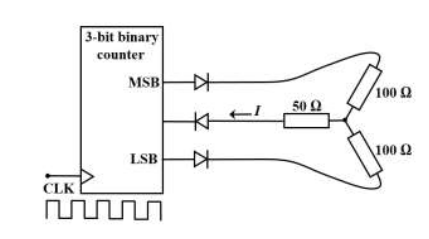
\includegraphics[width=\columnwidth]{figs/2018-gate-in-17.png}
\caption{}
\label{fig:2018-gate-in-17}
\end{figure}

   


\end{enumerate}


\end{document}
